\documentclass[10pt, compress]{beamer}

\usetheme[numbering=fraction, progressbar=none, titleformat=smallcaps, sectionpage=none]{metropolis}
\usepackage{booktabs}
\usepackage{array}
\usepackage{listings}
\usepackage{graphicx}
\usepackage[brazilian]{babel}
\usepackage[scale=2]{ccicons}
\usepackage{url}
\usepackage{relsize}
\usepackage{courier}

\usepackage{pgfplots}
\usepgfplotslibrary{dateplot}

\lstset{basicstyle=\footnotesize\ttfamily,breaklines=true}
\renewcommand*{\UrlFont}{\ttfamily\smaller\relax}

\graphicspath{{./img/}}

\title{Introdução à Programação de GPUs \\ com a Plataforma CUDA (Parte I)}
\author{\footnotesize Pedro Bruel \\ {\scriptsize phrb@ime.usp.br}}
\institute{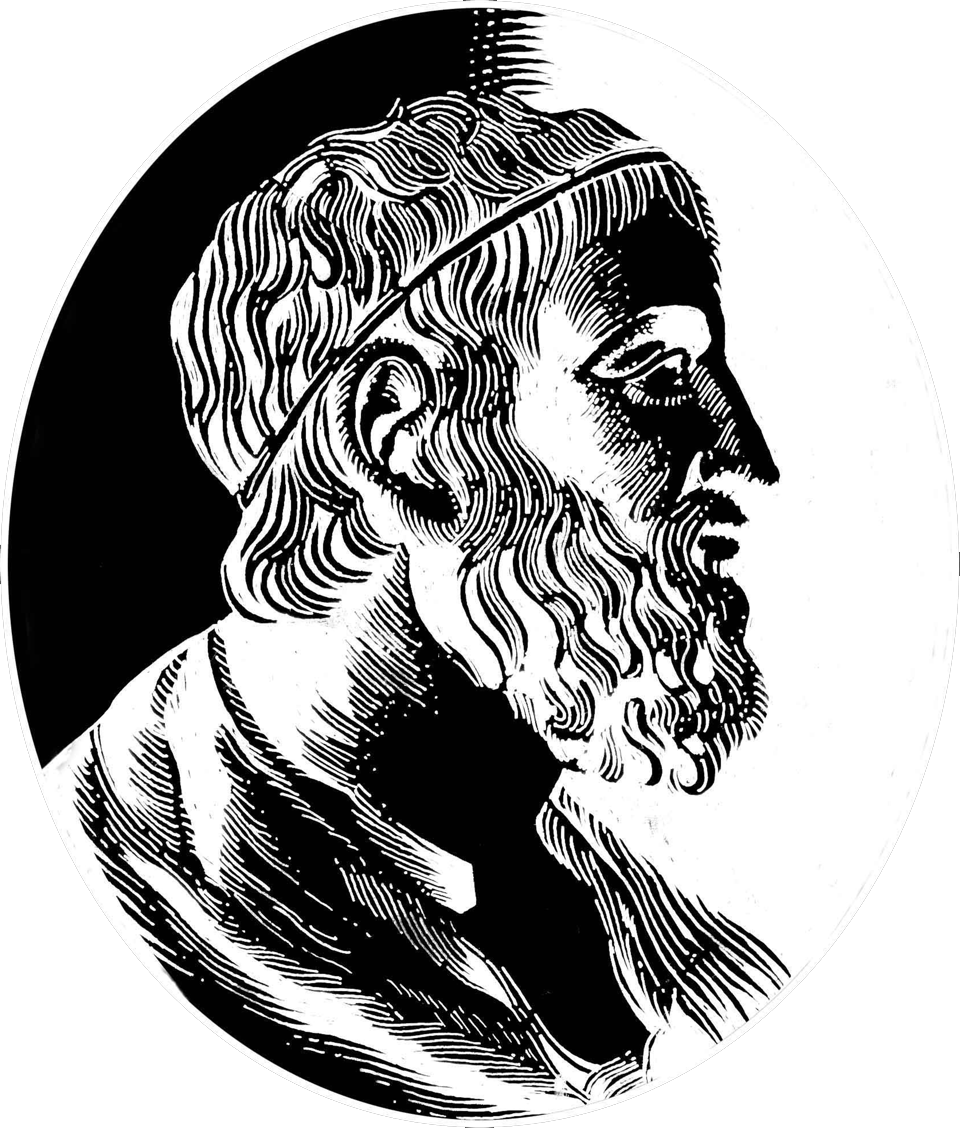
\includegraphics[height=2cm]{imelogo}\\[0.2cm] Instituto de Matemática e Estatística \\ Universidade de São Paulo}
\date{\scriptsize 04 de Agosto de 2016}

\begin{document}

\maketitle

\section{Apresentação}

\begin{frame}
    \frametitle{Roteiro}
    \setbeamertemplate{section in toc}[sections numbered]
    \begin{enumerate}
        \item Introdução
            \begin{itemize}
                \item Computação Heterogênea
                \item Escalabilidade e Portabilidade de Desempenho
            \end{itemize}
            \pause
        \item Programação em CUDA
            \begin{itemize}
                \item Diretivas de Compilador vs. Bibliotecas vs. Linguagens
                \item Alocação e Movimentação de Memória
                \item \emph{Threads} e \emph{Kernels}
            \end{itemize}
            \pause
        \item Exemplos
            \begin{itemize}
                \item Soma de vetores em CUDA C
                \item Mandelbrot em CUDA Python
            \end{itemize}
    \end{enumerate}
\end{frame}

\begin{frame}
    \frametitle{Recursos}

    Os \emph{pdf}s com as aulas e todo o código fonte usado nos exemplos estão
    no \alert{GitHub}:

    \begin{itemize}
        \item \url{github.com/phrb/aulas-gpu}
    \end{itemize}
    \pause

    Outros recursos:

    \begin{itemize}
        \item GPU Teaching Kit: \url{syllabus.gputeachingkit.com}
        \item iPython: \url{ipython.org/notebook.html}
        \item CUDA Toolkit: \url{developer.nvidia.com/cuda-toolkit}
        \item Anaconda: \url{continuum.io/downloads}
    \end{itemize}
\end{frame}

\begin{frame}
    \frametitle{Recursos}

    Os próximos \emph{slides} foram adaptados do
    material disponível no \alert{GPU Teaching Kit}:
    \begin{itemize}
        \item \url{syllabus.gputeachingkit.com}
    \end{itemize}

\end{frame}

\section*{Computação Heterogênea}

\begin{frame}
    \frametitle{Aceleração por \textit{Hardware}}
    Uso de \alert{dispositivos} para acelerar computações aplicadas a grandes
    conjuntos de dados:
    \begin{itemize}
        \item Associação a um processador \alert{hospedeiro}
            \pause
        \item Controle e memória próprios
            \pause
        \item Diferem em especialização e configurabilidade
            \pause
        \item \alert{GPUs}, DSPs, FPGAs, ASICs
    \end{itemize}
    \pause
    Casos de uso:
    \begin{itemize}
        \item Aprendizagem Computacional
        \item Processamento Digital de Sinais e Imagens
        \item Bioinformática
        \item Criptografia
        \item Simulações
        \item ...
    \end{itemize}
\end{frame}

\begin{frame}
    \frametitle{Aceleração por \textit{Hardware}}
    \centering
    
\includegraphics[width=.8\textwidth]{accel}
\end{frame}

\begin{frame}
    \frametitle{Aceleração por \textit{Hardware}}
    Porcentagem de sistemas com aceleradores na \textit{Top500}:

    \begin{center}
    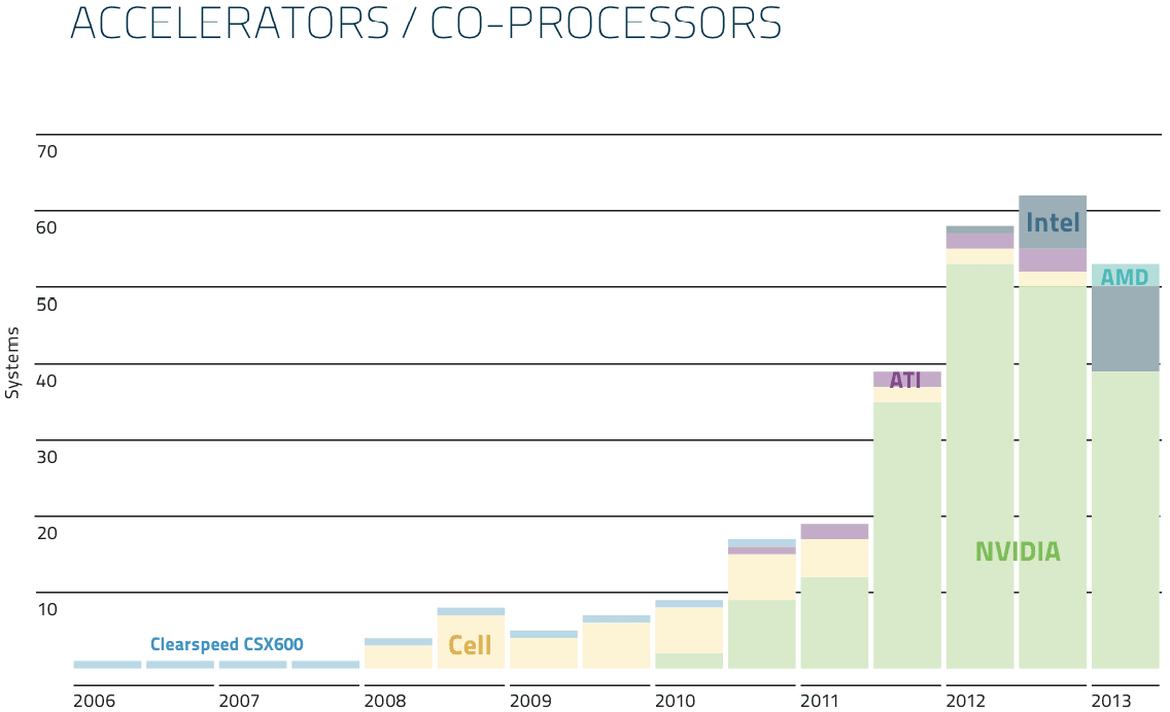
\includegraphics[width=.85\textwidth]{top500_accel}
    \hfill

    \tiny{Imagem: \url{cnet.com/pictures/top500-supercomputing-trends-visualized-pictures} [Acessado em 29/07/16]}
    \end{center}
\end{frame}

\begin{frame}
    \frametitle{Computação Heterogênea}
    Dados recursos computacionais \alert{heterogêneos}, conjuntos de
    \alert{dados} e \alert{computações}, como distribuir computações e dados de
    forma a \alert{otimizar o uso} dos recursos?
\end{frame}

\begin{frame}
    \frametitle{Computação Heterogênea}
    Recursos computacionais \alert{heterogêneos}:
    \begin{itemize}
        \item Baixa Latência: CPUs
        \item Alta Vazão: GPUs
        \item Reconfiguráveis: FPGAs
        \item Especializados: ASICs, DSPs
    \end{itemize}
    \pause
    Conjuntos de \alert{dados}:
    \begin{itemize}
        \item \textit{Big Data}
        \item \textit{Data Streams}
        \item ...
    \end{itemize}
    \pause
    \alert{Computações}:
    \begin{itemize}
        \item \textit{MapReduce}
        \item \textit{Task Parallelism}
        \item ...
    \end{itemize}
\end{frame}

\begin{frame}
    \frametitle{Computação Heterogênea}
    \centering
    
\includegraphics[width=.85\textwidth]{heterogeneous}
\end{frame}

\section*{GPUs}

\begin{frame}
    \frametitle{Modelo de \textit{Hardware}}
    Taxonomia de Flynn:
    \begin{itemize}
        \item \textit{Single Instruction Multiple Data} (SIMD)
    \end{itemize}
    \pause
    Escalonamento e execução:
    \begin{itemize}
        \item \textit{Streaming Multiprocessor} (SM)
        \item \textit{Warps, Grids, Blocks} e \textit{Threads}
    \end{itemize}
    \pause
    Escalonamento de mais alto-nível:
    \begin{itemize}
        \item \textit{Graphics Processing Cluster} (GPC)
        \item \textit{Texture Processor Cluster} (TPC)
    \end{itemize}
    \pause
    Memória:
    \begin{itemize}
        \item Compartilhada: Cache L1, L2; \textit{megabytes} (Nvidia Pascal)
        \item Global: GDDR5; \textit{gigabytes}
            \pause
        \item SSD: \alert{\textit{terabytes}} (AMD Polaris)
    \end{itemize}
\end{frame}

\begin{frame}
    \frametitle{Arquitetura Pascal GP100}
    \centering
    \includegraphics[width=.65\textwidth]{gp100_view}
    \hfill

    \tiny{Imagem: \url{images.nvidia.com/content/pdf/tesla/whitepaper/pascal-architecture-whitepaper.pdf} [Acessado em 29/07/16]}
\end{frame}

\begin{frame}
    \frametitle{Arquitetura Pascal GP100: \textit{Compute Capability 6.0}}
    \centering
    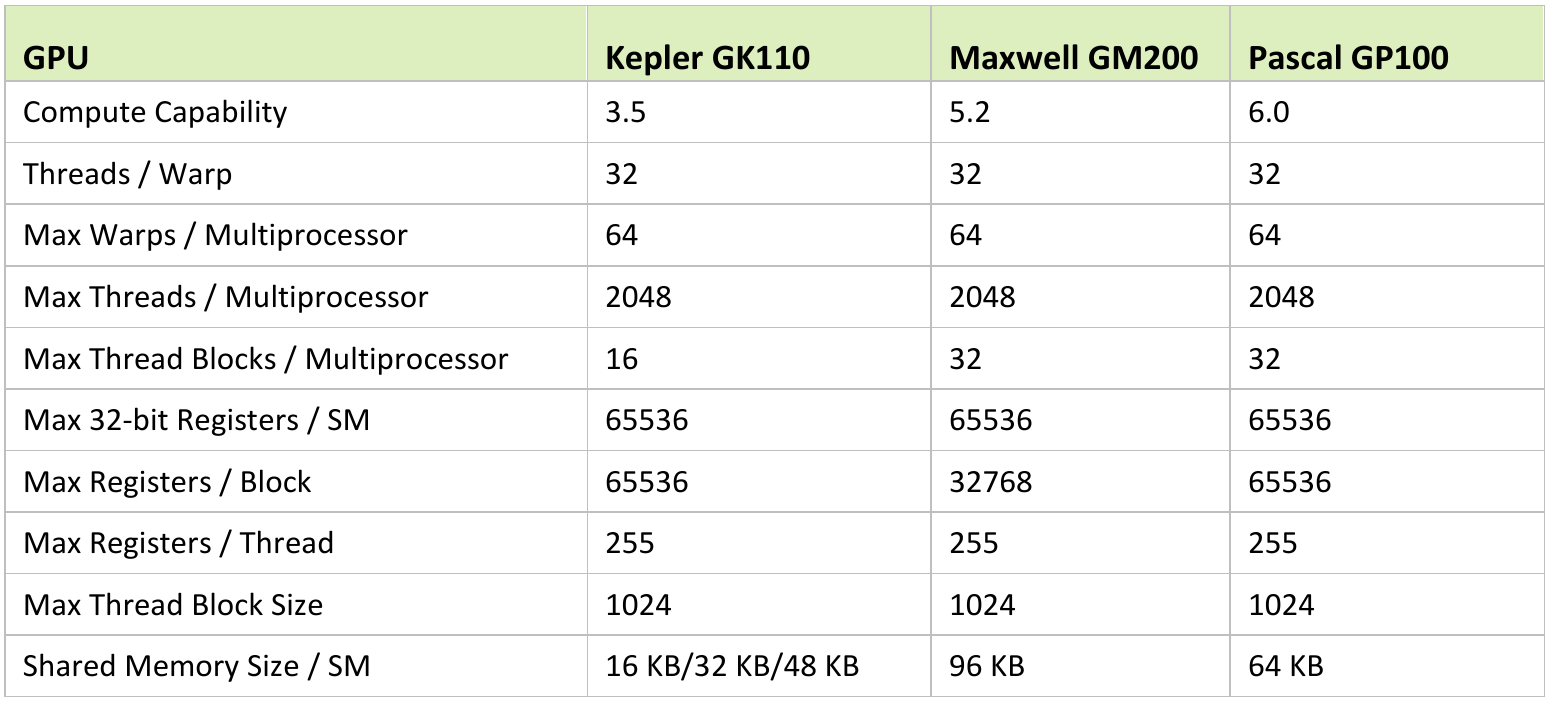
\includegraphics[width=\textwidth]{cc_6}
    \hfill

    \tiny{Imagem: \url{images.nvidia.com/content/pdf/tesla/whitepaper/pascal-architecture-whitepaper.pdf} [Acessado em 29/07/16]}
\end{frame}

\begin{frame}
    \frametitle{Arquitetura Pascal GP100: \textit{Compute Capability 6.0}}
    \centering
    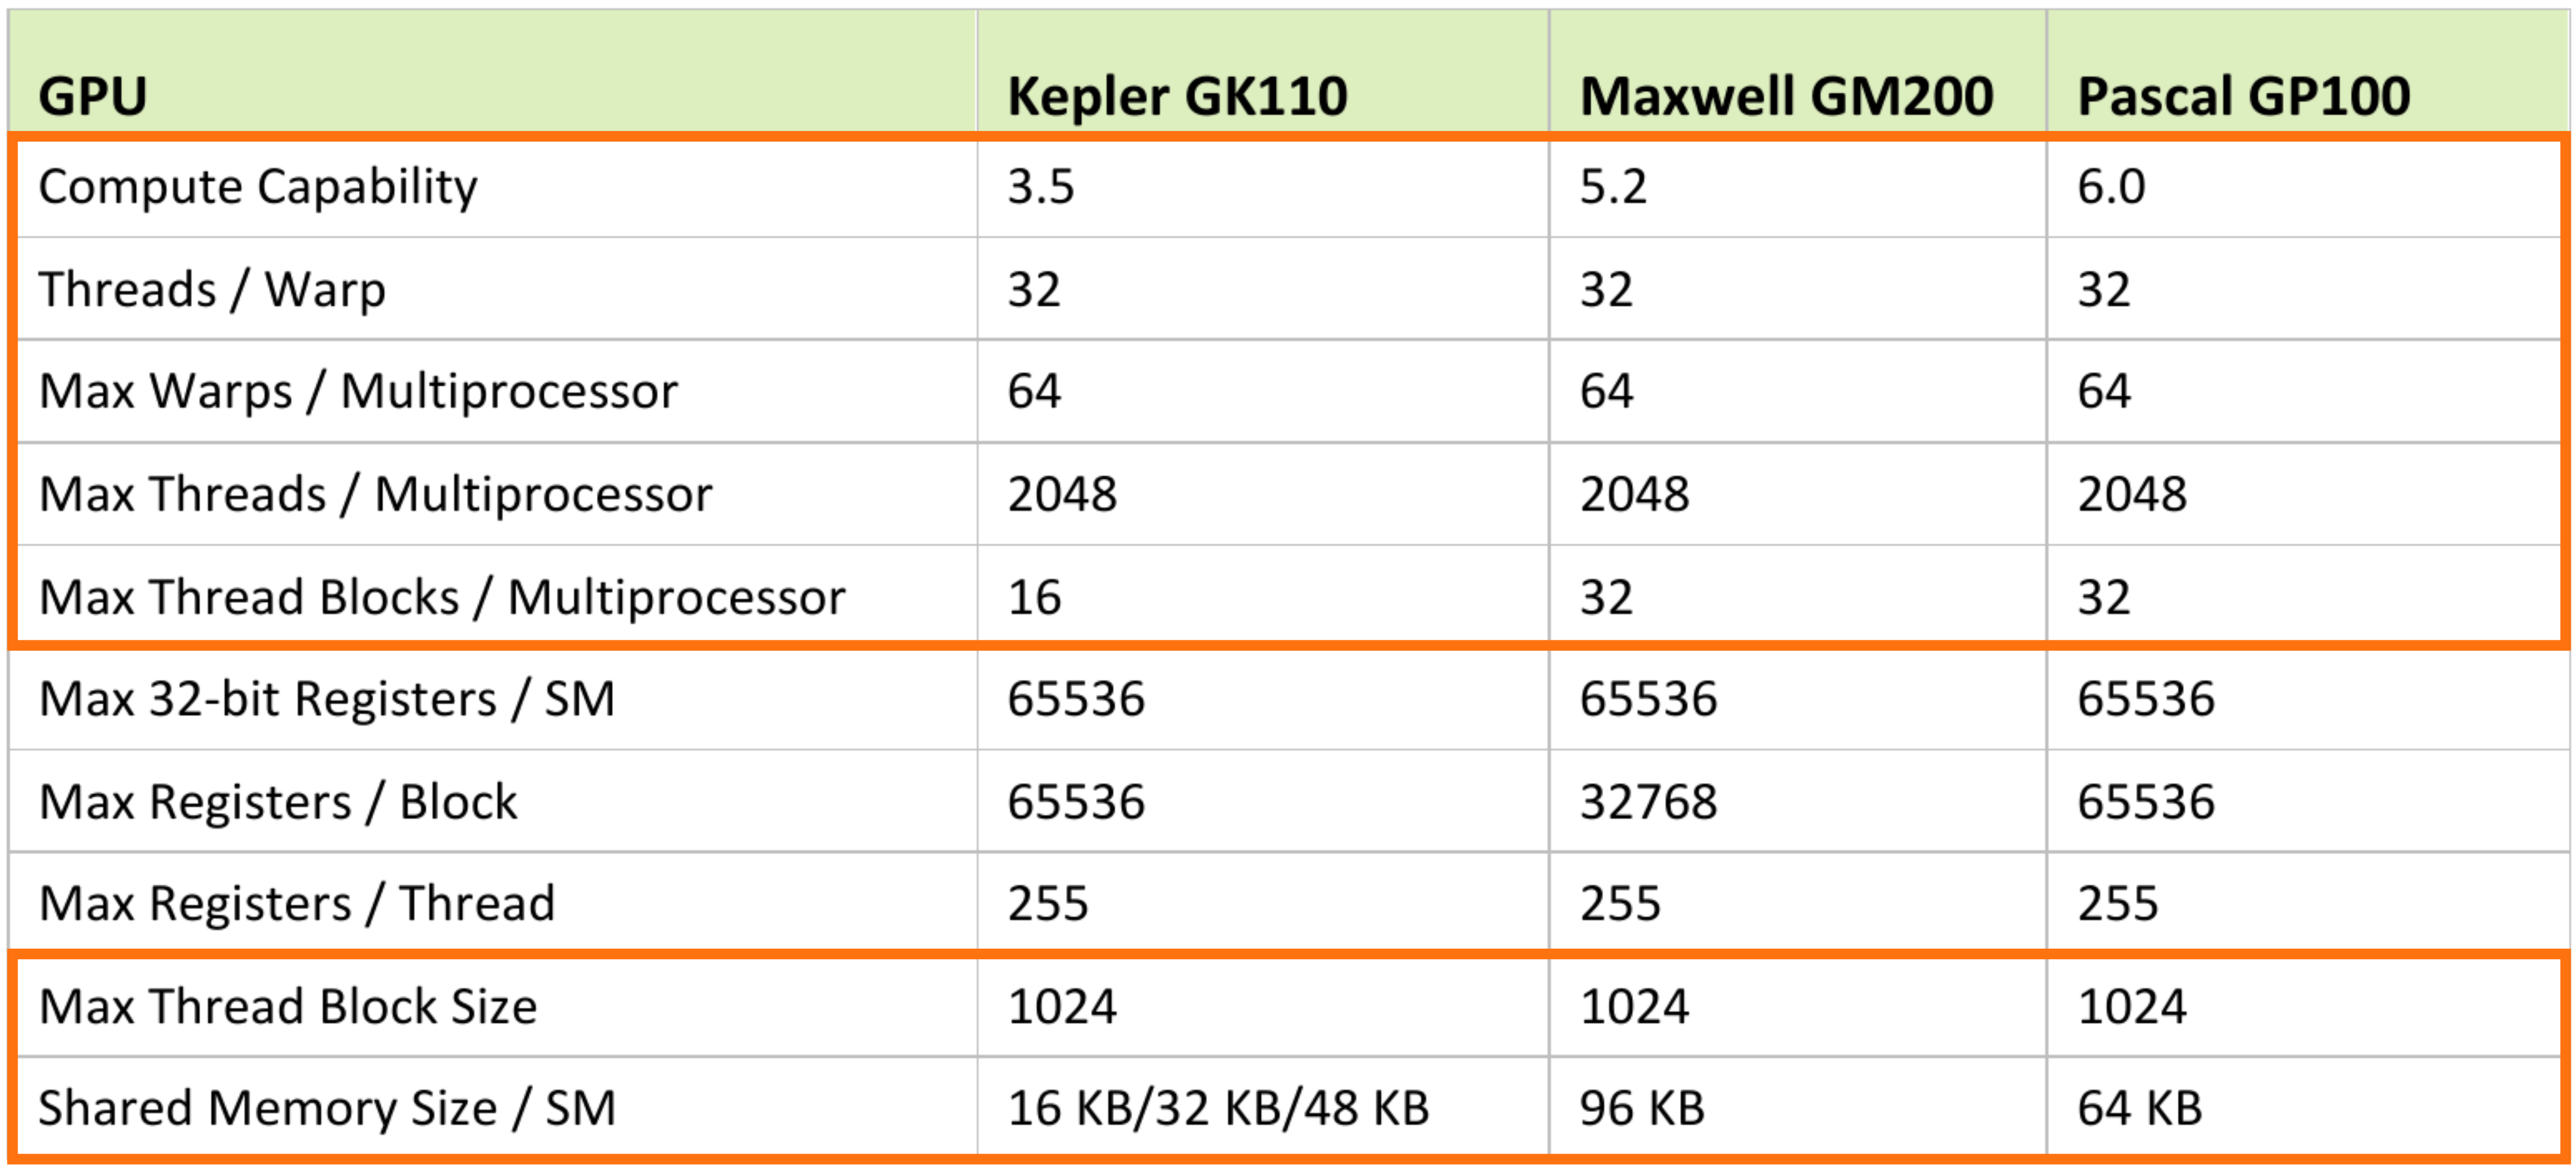
\includegraphics[width=\textwidth]{cc_6_highlight}
    \hfill

    \tiny{Imagem: \url{images.nvidia.com/content/pdf/tesla/whitepaper/pascal-architecture-whitepaper.pdf} [Acessado em 29/07/16]}
\end{frame}

\begin{frame}
    \frametitle{Arquitetura Pascal GP100: SM}
    \centering
    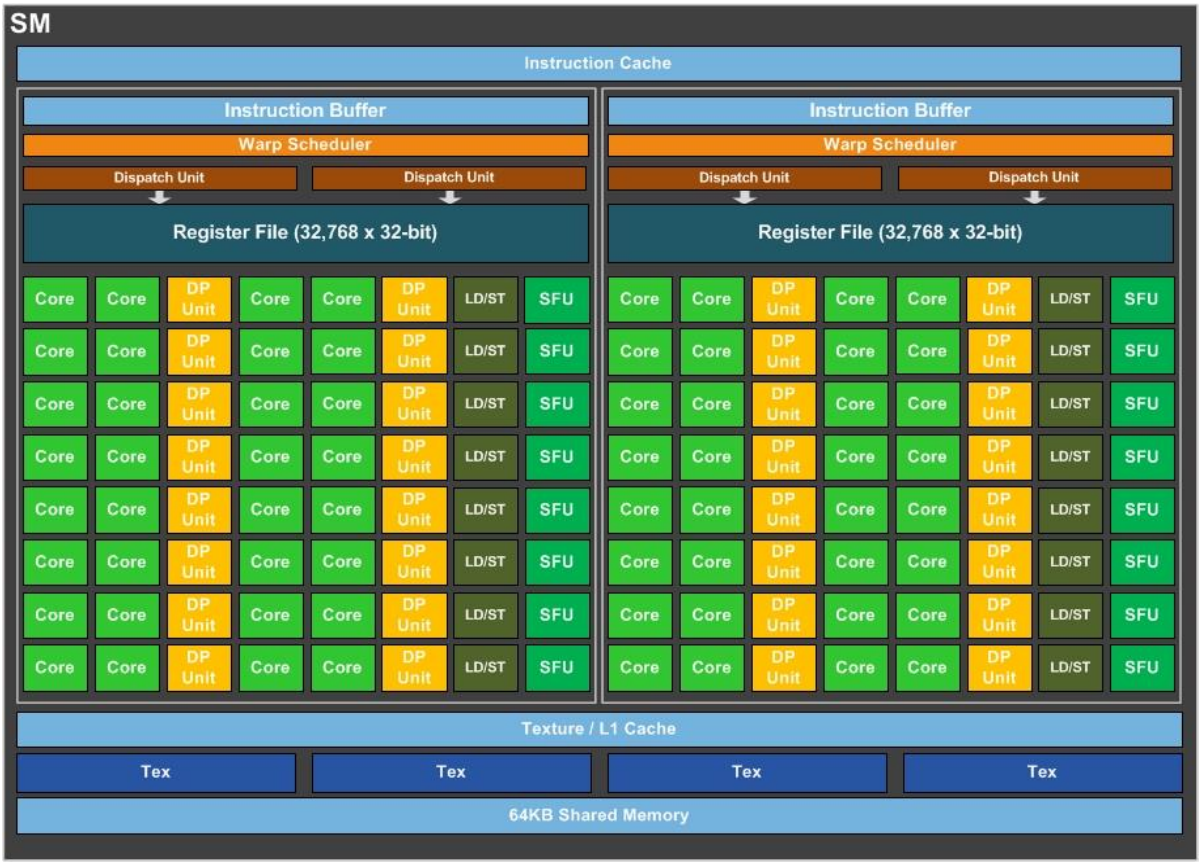
\includegraphics[width=.9\textwidth]{gp100_SM_diagram}
    \hfill

    \tiny{Imagem: \url{images.nvidia.com/content/pdf/tesla/whitepaper/pascal-architecture-whitepaper.pdf} [Acessado em 29/07/16]}
\end{frame}

\begin{frame}
    \frametitle{Arquitetura Pascal GP100}
    \centering
    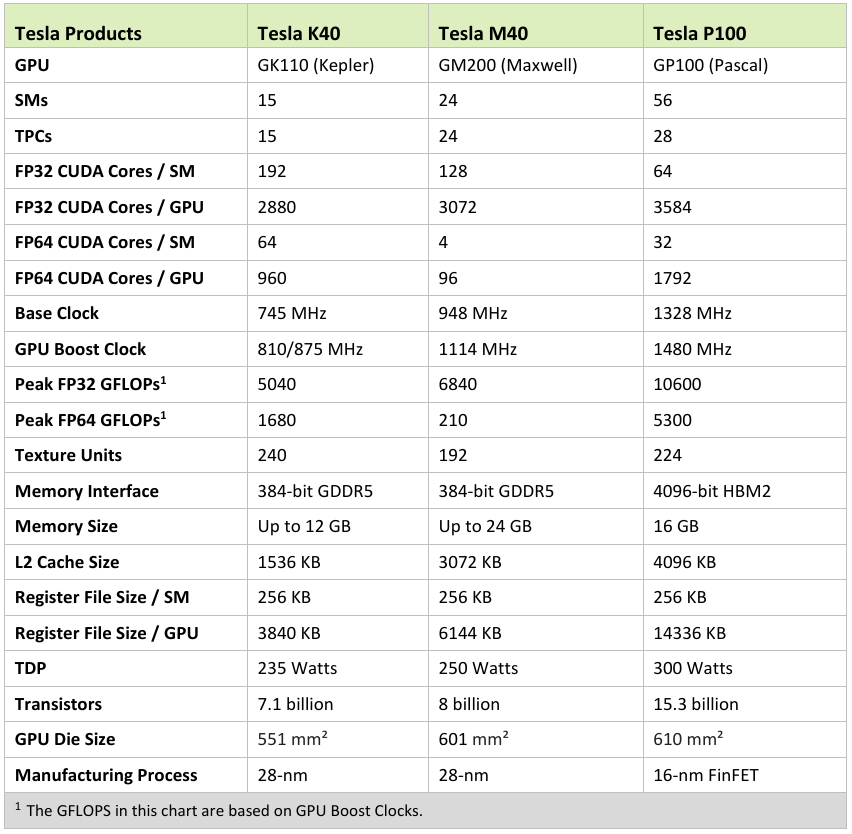
\includegraphics[width=.7\textwidth]{gp100_stats}
    \hfill

    \tiny{Imagem: \url{images.nvidia.com/content/pdf/tesla/whitepaper/pascal-architecture-whitepaper.pdf} [Acessado em 29/07/16]}
\end{frame}

\begin{frame}
    \frametitle{Arquitetura Pascal GP100}
    \centering
    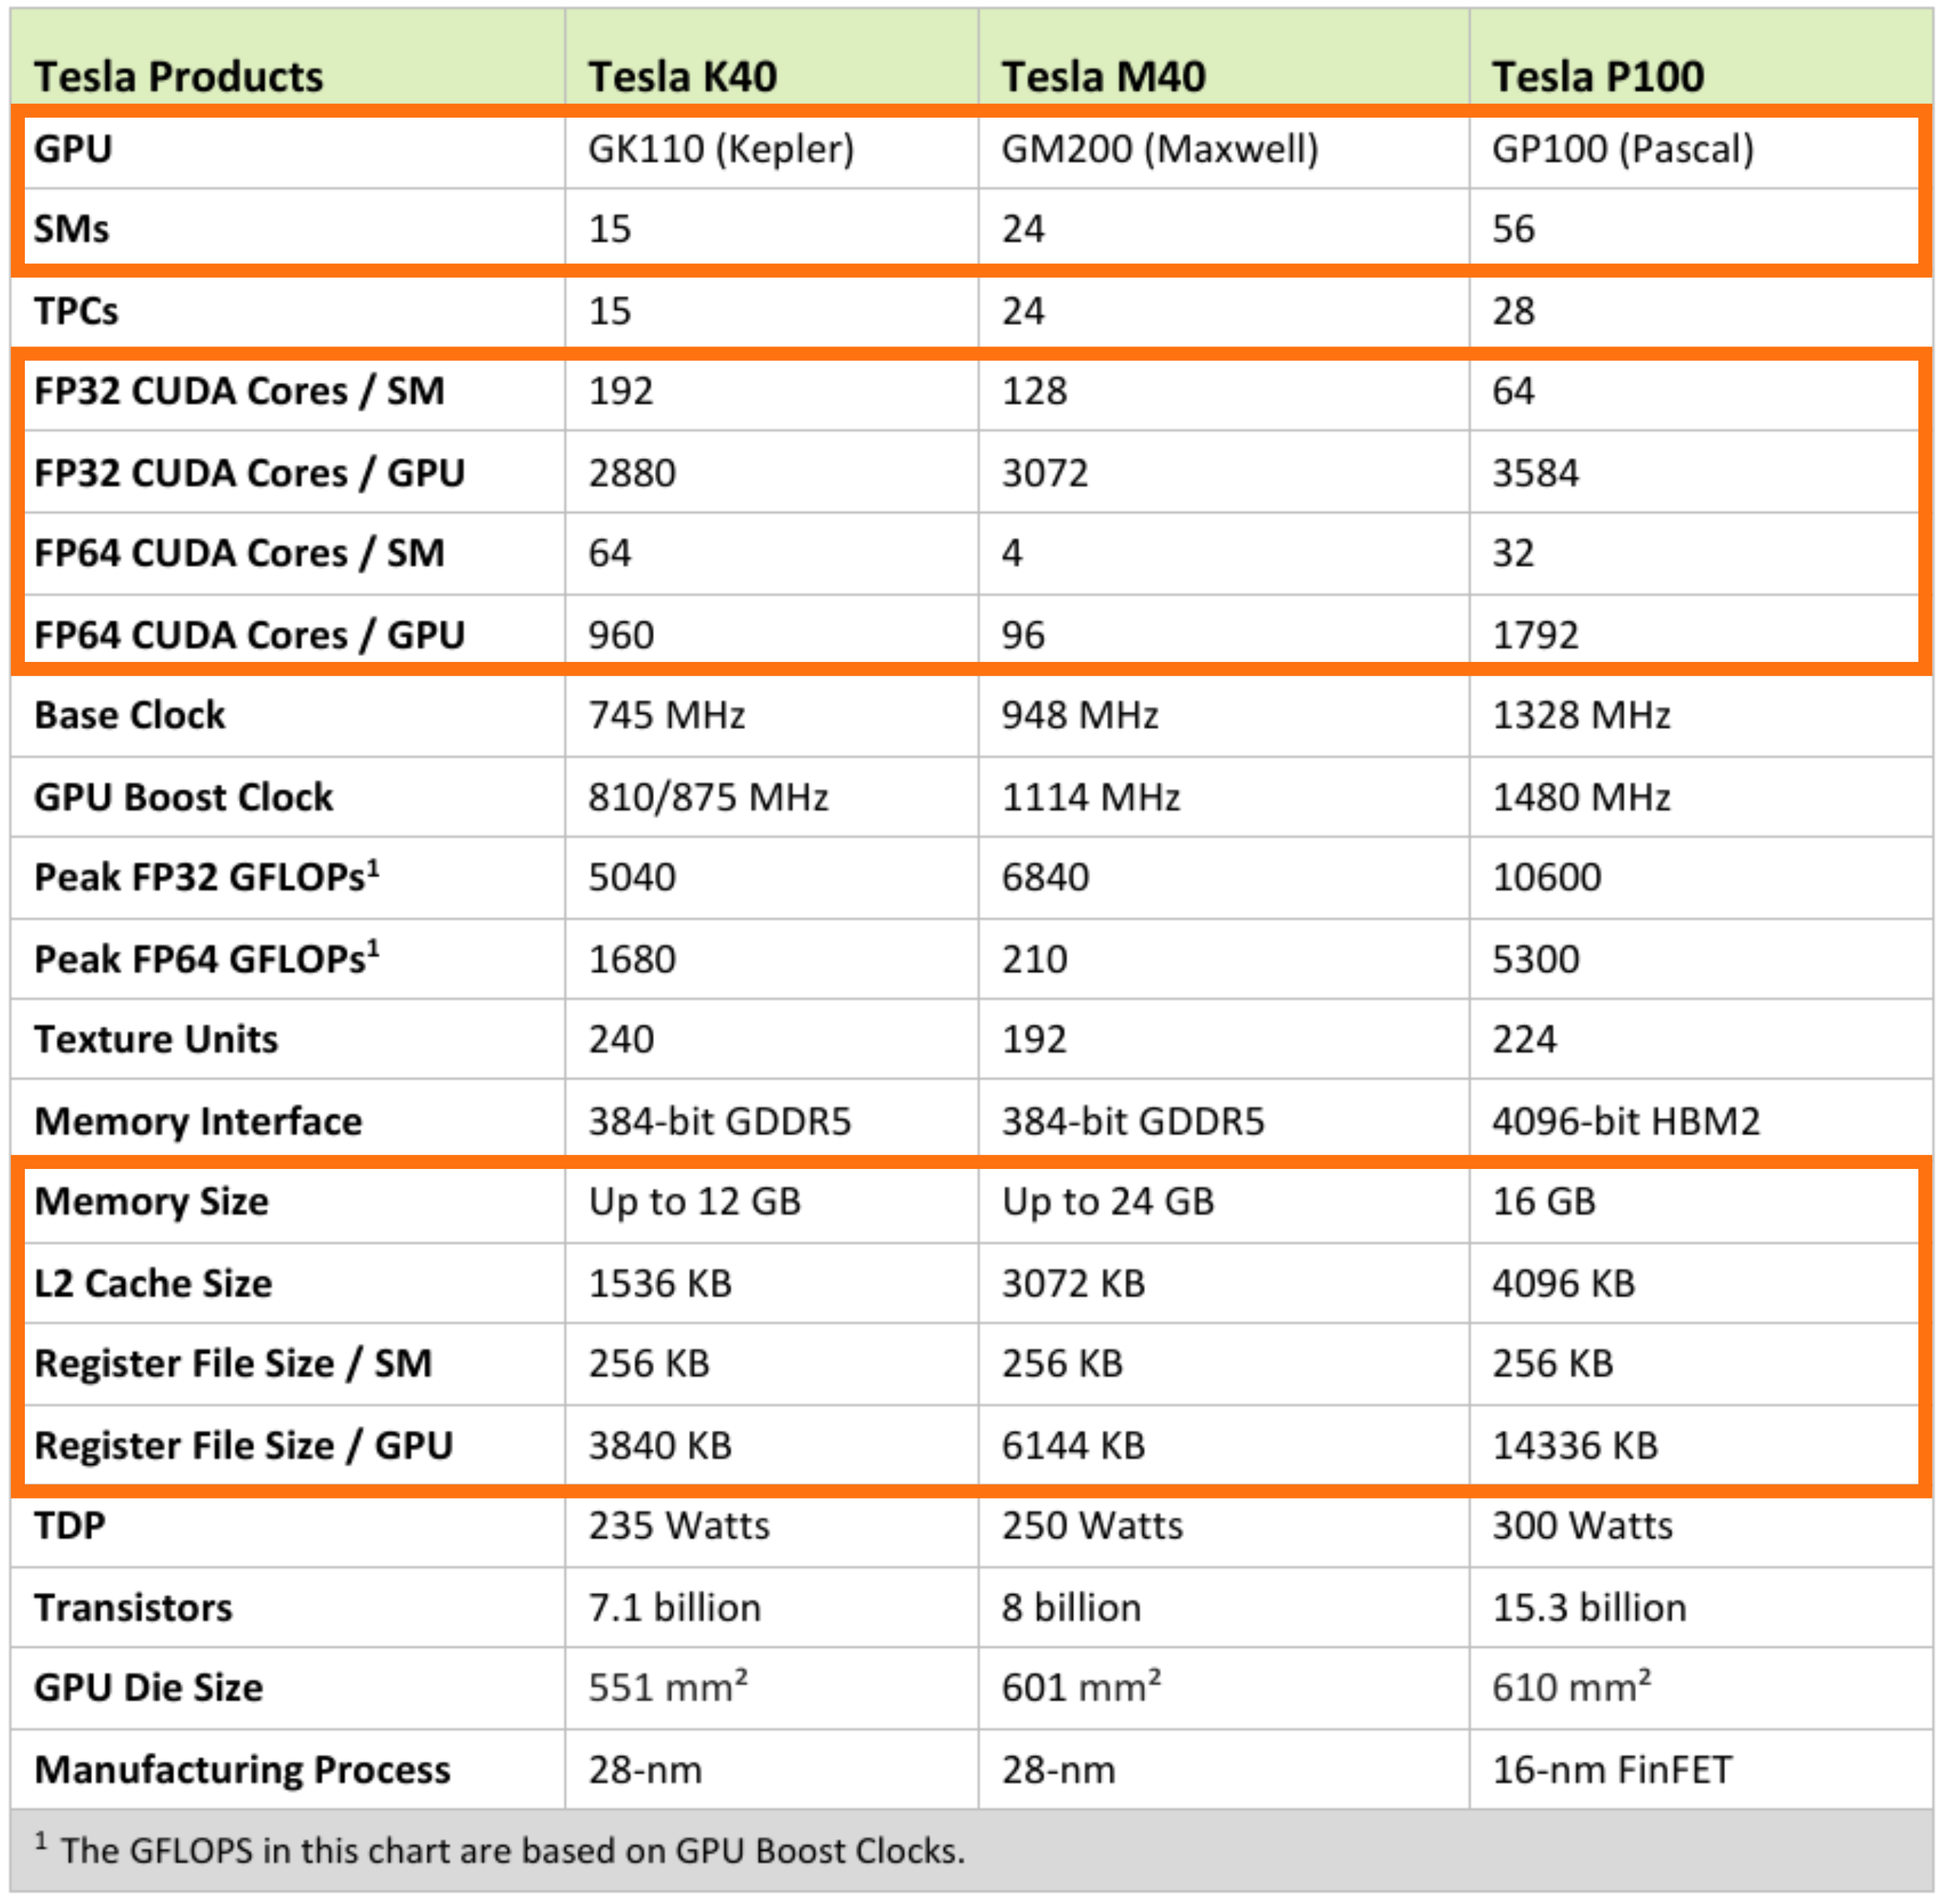
\includegraphics[width=.7\textwidth]{gp100_stats_highlight}
    \hfill

    \tiny{Imagem: \url{images.nvidia.com/content/pdf/tesla/whitepaper/pascal-architecture-whitepaper.pdf} [Acessado em 29/07/16]}
\end{frame}

\begin{frame}
    \frametitle{Arquitetura Pascal GP100}
    \centering
    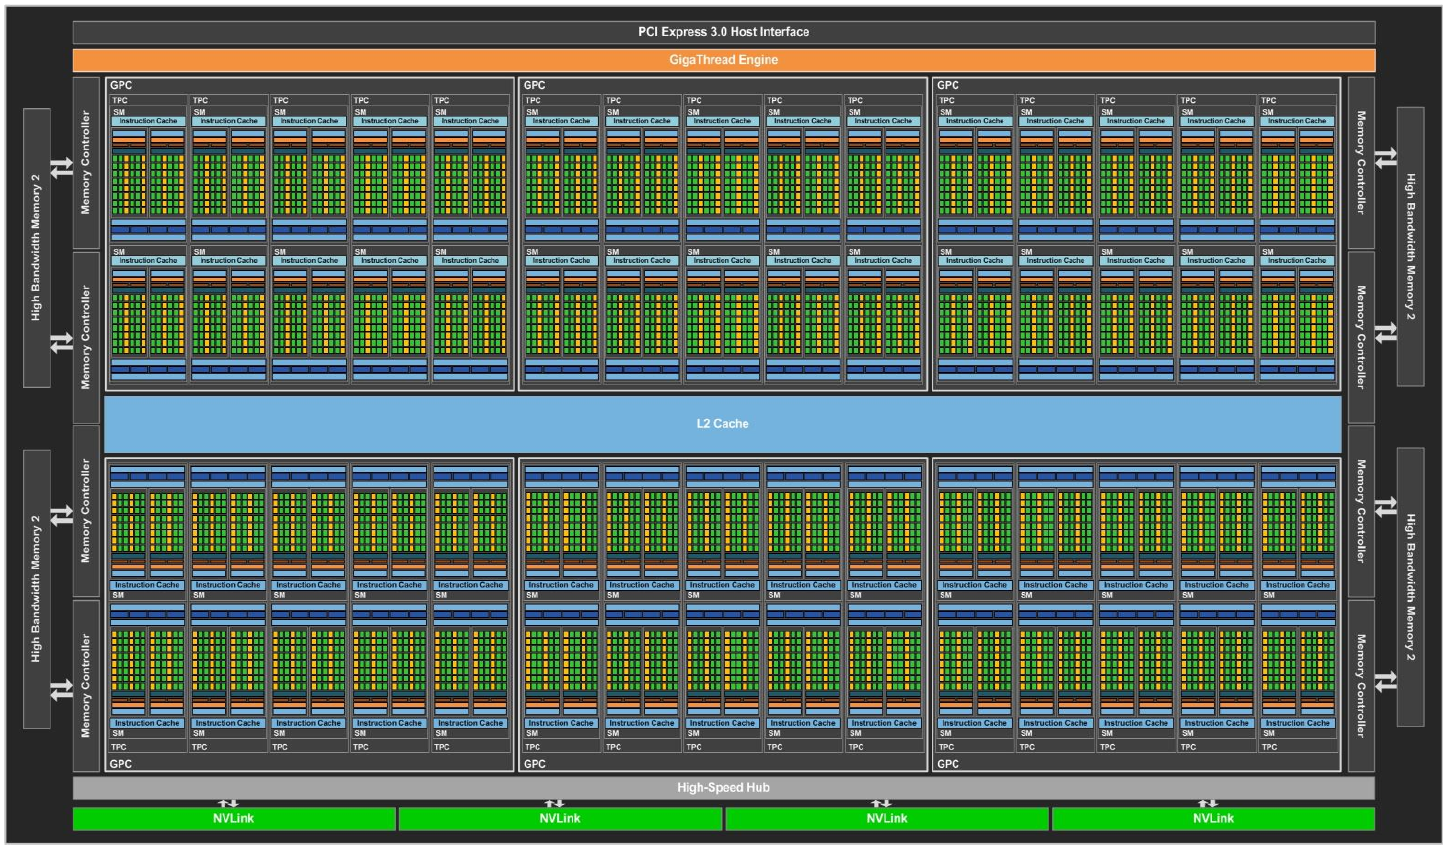
\includegraphics[width=.95\textwidth]{gp100_diagram}
    \hfill

    \tiny{Imagem: \url{images.nvidia.com/content/pdf/tesla/whitepaper/pascal-architecture-whitepaper.pdf} [Acessado em 29/07/16]}
\end{frame}

\maketitle

\end{document}
